\section{Divisori di frequenza}
\subsection{Montaggio e verifica}
Si è innanzitutto realizzato il circuito in \fig{div} utilizzando l'integrato SN74LS93 (un ripple counter costituito da quattro JK flip-flop), mettendo uno degli ingressi di reset ($R_{0,1}$) a terra, per poi verificarne visivamente il corretto funzionamento inviando un clock lento ($\sim \SI{1}{\Hz}$) ed osservando i LED (e dunque gli output dei flip-flop) "contare" ciclicamente da 0 a 15.

\begin{figure}[h]
	\centering
	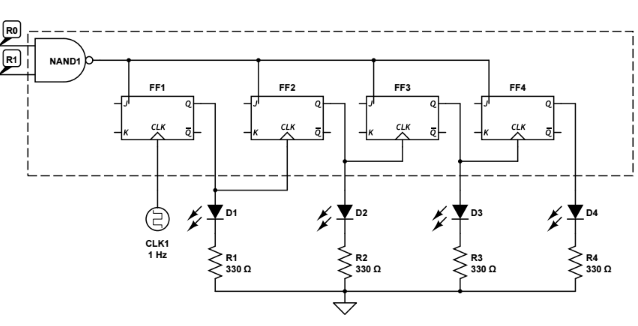
\includegraphics[scale=0.8]{divisori.png}
	\caption{Circuito divisore}
	\label{fig:div}
\end{figure}

\subsection{Verifica funzionamento divisore e misura dei tempi di ritardo.}
Effettuata la verifica precedente si è posta $f_{clock} = \SI{49.998(1)}{ \kilo \hertz}$ per procedere dunque alla misura della frequenza dei segnali in uscita ai flip-flop del contatore, ottenendo i valori in \tab{divlag}.

I segnali sono riportati in \fig{divout}. Si ha dunque come atteso un funzionamento da divisore di frequenza (con ottima precisione).

\begin{figure}[h]
	\centering
	\begin{minipage}{0.47\textwidth}
		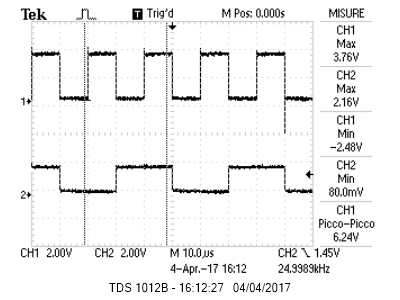
\includegraphics[scale=0.8]{divisore_2x.png}
		\\
		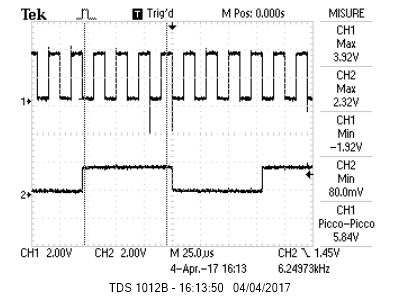
\includegraphics[scale=0.8]{divisore_8x.png}
	\end{minipage}
	\begin{minipage}{0.47\textwidth}
		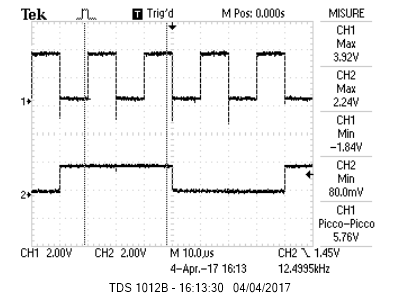
\includegraphics[scale=0.8]{divisore_4x.png}
		\\
		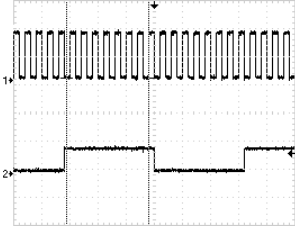
\includegraphics[scale=0.8]{divisore_16x.png}
	\end{minipage}
	\caption{Output dei quattro flip-flop del divisore (CH2) e segnale di clock (CH1).}
	\label{fig:divout}
\end{figure}

Si sono successivamente misurati i tempi di ritardo degli output dei flip-flop, ovvero l'intervallo temporale tra il fronte (di discesa) del clock in cui ci si attende una variazione dell'output e il fronte della variazione stessa, misurato tra i punti di tensione intermedia tra il livello alto e quello basso. I valori ottenuti sono riportati in \tab{divlag}.

\begin{table}[h]
	\centering
	\begin{tabular}{l S[table-figures-decimal=4, table-figures-uncertainty=1] S[table-figures-decimal=1, table-figures-integer=3, table-figures-uncertainty=1] S[table-figures-decimal=1, table-figures-uncertainty=1] }
		\toprule
			& {$f$ [\si{\kHz}]} & {$\Delta t_{salita}$ [\si{\ns}]} & {$\Delta t_{discesa}$ [\si{\ns}]} \\
		\midrule
		$Q_1$ & 24.999(1) & 76.0(4) & 24.2(1) \\
		$Q_2$ & 12.499(1) & 101 (1) & 30.8(2) \\
		$Q_3$ & 6.2497(1) & 110 (1) & 42.0(2) \\
		$Q_4$ & 3.1251(1) & 155 (1) & 53.2(4) \\
		\bottomrule
	\end{tabular}
	\caption{Tempi di ritardo e frequenze misurate per il circuito divisore.}
	\label{tab:divlag}
\end{table}

\paragraph{Costruzione circuito di reset}
Per realizzare un sistema di reset per circuito divisore
è stato montato il contatore asincrono in \figurename{  \ref{f:reset} }.
Per tale circuito è stata lasciata flottante l'ingresso $R1$
